\documentclass[a4j]{jarticle}

\usepackage[dvipdfmx]{graphicx}
\usepackage{epsbox}
\usepackage{url}
\usepackage{here}

\setlength{\headsep}{-5mm}
\setlength{\oddsidemargin}{0mm}
\setlength{\textwidth}{165mm}
\setlength{\textheight}{230mm}
\setlength{\footskip}{20mm}

\title{
\vspace{30mm}
{\bf データテーブル}
\date{}
}

\begin{document}
\maketitle
\section{データベース設計}
本章では、システムで用いるデータベースの設計について記します。
\subsection{データテーブル相関図}
本小節では、テーブル間の関係性をER図を用いて示します。
\begin{figure}[H]
  \begin{center} %センタリングする
    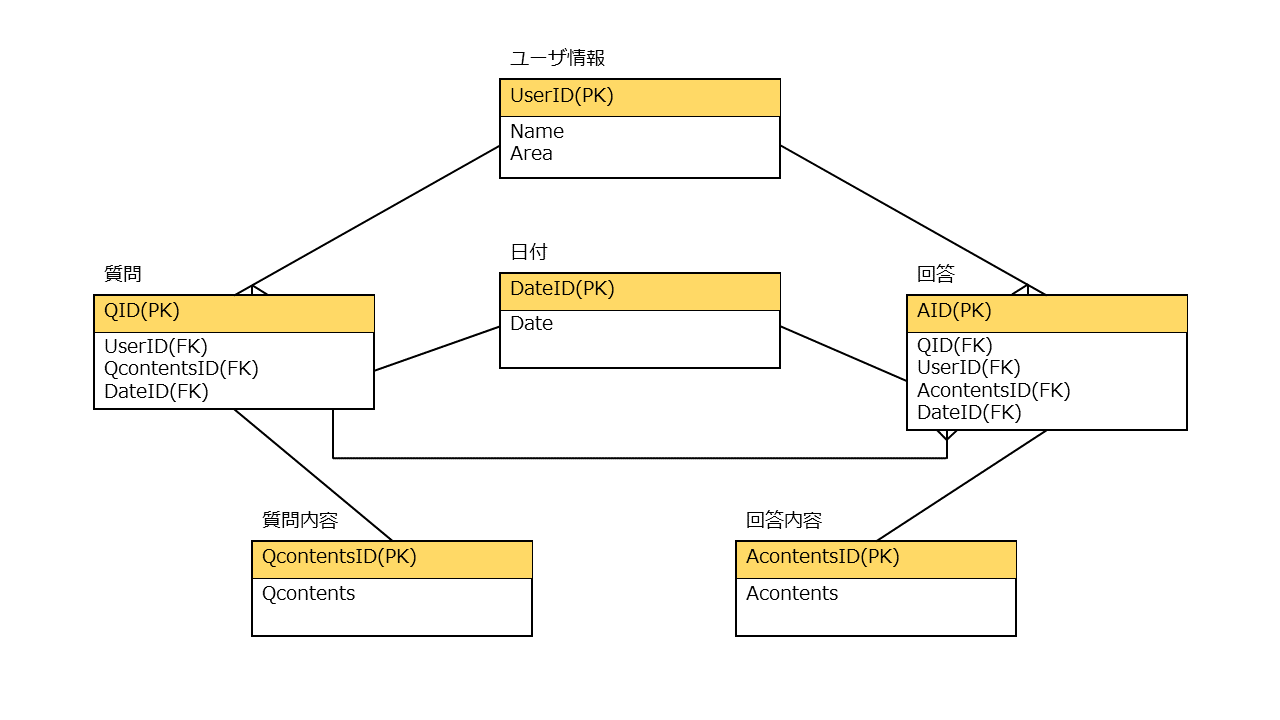
\includegraphics[width=16.0cm]{ER図.png}
    \caption{データテーブルER図} %タイトルをつける
    \label{fig:er} %ラベルをつけ図の参照を可能にする
  \end{center}
\end{figure}

今回用いるデータベースシステムでは、ユーザ情報の定義と質問箱の管理を行っています。\\
図\ref{fig:er}のように、親ユーザと質問・回答の関係性、質問と回答の関係性はそれぞれ1対多の関係性になっており、それ以外のテーブルは1対1の関係性となっています。

%ユーザ情報 -> アカウント情報に変えたほうがいい??????
\subsection{データテーブル設計}
本小節では、それぞれのデータテーブルの詳細について記します。

\subsubsection{ユーザ情報}

\begin{table}[H]
    \caption{ユーザ情報}
    \label{tbl: user}
    \begin{center}
        \begin{tabular}{|c|c|c|c|c|c|} \hline
            属性 & データ型 & データ長 & SQLite & key:Table名 & NULL\\ \hline \hline
            UserID & 半角英数字型 & 6文字固定長 & TEXT & PK & Not\\ \hline
            Name & 全角文字型 & 10文字可変長 & TEXT & & Not\\ \hline
            Area & 全角文字型 & 5文字可変長 & TEXT & & Not\\ \hline
        \end{tabular}
    \end{center}
\end{table}

表\ref{tbl: user}ではユーザ情報を格納しています。ユーザIDと名前、住んでいる地域を管理することで、質問箱でどの地域の人が投稿を行っているのか分かるようにしています。\\
各フィールドの概要は以下の通りです。
\begin{itemize}
  \item ユーザID(UserID):
  ユーザテーブルの主キー
  \item ユーザ名(Name):
  ユーザの名前
  \item 居住地域名(Area):
  ユーザが住んでいる地域名
\end{itemize}

\subsubsection{質問テーブル}

\begin{table}[H]
    \caption{質問}
    \label{tbl: question}
    \begin{center}
        \begin{tabular}{|c|c|c|c|c|c|} \hline
            属性 & データ型 & データ長 & SQLite & key:Table名 & NULL\\ \hline \hline
            QID & 半角英数字型 & 8文字固定長 & TEXT & PK & Not\\ \hline
            UserID & 半角英数字型 & 6文字固定長 & TEXT & FK:親ユーザー情報 & Not\\ \hline
            QcontentsID & 半角英数字型 & 10文字固定長 & TEXT & FK:質問内容 & Not\\ \hline
            DateID & 半角英数字型 & 8文字固定長 & TEXT & FK:日付 & Not\\ \hline
        \end{tabular}
    \end{center}
\end{table}

表\ref{tbl: question}では、質問と質問者の関連付けを行っています。質問IDを主キーとし、ユーザ情報テーブル、質問内容テーブル、日付テーブルといったテーブルの主キーを外部キーとすることで、質問を投稿、確認できるようにしています。\\
各フィールドの概要は以下の通りです。
\begin{itemize}
  \item 質問ID(QID):
  質問テーブルの主キー
  \item ユーザID(UserID):
  ユーザテーブルの主キー
  \item 質問内容ID(QcontentsID):
  質問内容テーブルの主キー
  \item 日付ID(DateID):
  日付テーブルの主キー
\end{itemize}

\subsubsection{回答テーブル}
\begin{table}[H]
    \caption{回答}
    \label{tbl: answer}
    \begin{center}
        \begin{tabular}{|c|c|c|c|c|c|} \hline
            属性 & データ型 & データ長 & SQLite & key:Table名 & NULL\\ \hline \hline
            AID & 半角英数字型 & 8文字固定長 & TEXT & PK & Not\\ \hline
            QID & 半角英数字型 & 8文字固定長 & TEXT & FK:質問 & Not\\ \hline
            UserID & 半角英数字型 & 6文字固定長 & TEXT & FK:親ユーザー情報 & Not\\ \hline
            AcontentsID & 半角英数字型 & 10文字固定長 & TEXT & FK:回答内容 & Not\\ \hline
            DateID & 半角英数字型 & 8文字固定長 & TEXT & FK:日付 & Not\\ \hline
        \end{tabular}
    \end{center}
\end{table}
表\ref{tbl: answer}では、回答と回答者の関連付けを行っています。回答IDを主キーとし、質問テーブルと同様に外部キーを指定しています。また、質問テーブルも外部キーとしています。これにより、一つの質問に対して、複数の回答を関連付けることができます。\\
各フィールドの概要は以下の通りです。
\begin{itemize}
  \item 回答ID(AID):
  回答テーブルの主キー
  \item 質問ID(QID):
  質問テーブルの主キー
  \item ユーザID(UserID):
  ユーザテーブルの主キー
  \item 回答内容ID(AcontentsID):
  回答内容テーブルの主キー
  \item 日付ID(DateID):
  日付テーブルの主キー
\end{itemize}

\subsubsection{質問内容テーブル}
\begin{table}[H]
    \caption{質問内容}
    \label{tbl: qcontents}
    \begin{center}
        \begin{tabular}{|c|c|c|c|c|c|} \hline
           属性 & データ型 & データ長 & SQLite & key:Table名 & NULL\\ \hline \hline
            QcontentsID & 半角英数字型 & 10文字固定長 & TEXT & PK & Not\\ \hline
            Qcontents & 全角文字型 & 1000文字可変長 & TEXT & & Not\\ \hline
        \end{tabular}
    \end{center}
\end{table}
表\ref{tbl: qcontents}では、質問内容を管理を行っています。質問内容の本文は全角文字型で1000文字まで投稿することができます。質問内容と質問を分けて管理することで、データの正規化を図っています。\\
各フィールドの概要は以下の通りです。
\begin{itemize}
  \item 質問内容ID(QcontentsID):
  質問内容テーブルの主キー
  \item 質問内容(Qcontents):
  質問内容の本文
\end{itemize}

\subsubsection{回答内容テーブル}
\begin{table}[H]
    \caption{回答内容}
    \label{tbl: acontents}
    \begin{center}
        \begin{tabular}{|c|c|c|c|c|c|} \hline
            属性 & データ型 & データ長 & SQLite & key:Table名 & NULL\\ \hline \hline
            AcontentsID & 半角英数字型 & 10文字固定長 & TEXT & PK & Not\\ \hline
            Acontents & 全角文字型 & 1000文字可変長 & TEXT & & Not\\ \hline
        \end{tabular}
    \end{center}
\end{table}
表\ref{tbl: acontents}では回答内容を管理を行っています。質問内容テーブルと同様に、回答内容の本文も全角文字型で1000文字まで投稿できます。\\
各フィールドの概要は以下の通りです。
\begin{itemize}
  \item 回答内容ID(AcontentsID):
  回答内容テーブルの主キー
  \item 回答内容(Acontents):
  回答内容の本文
\end{itemize}
%日付テーブル消して質問と回答にくっつけたほうが良い気がしてきた
\subsubsection{日付}
\begin{table}[H]
    \caption{日付}
    \label{tbl: date}
    \begin{center}
        \begin{tabular}{|c|c|c|c|c|c|} \hline
            属性 & データ型 & データ長 & SQLite & key:Table名 & NULL\\ \hline \hline
            DateID & 半角英数字型 & 8文字固定長 & TEXT & PK & Not\\ \hline
            Date & 日付型 & 20文字固定長 & NUMERIC & & Not\\ \hline
        \end{tabular}
    \end{center}
\end{table}
表\ref{tbl: date}では日付の管理を行っています。日付はIDで管理されており、呼び出したIDから日付を取得します。日付は日付型で管理されています。\\
各フィールドの概要は以下の通りです。
\begin{itemize}
  \item 日付ID(DateID):
  日付テーブルの主キー
  \item 日付(Date):
  日付と時刻の保存
\end{itemize}

\end{document}
